\clearpage
\section{考察}
\subsection{課題考察}
\begin{enumerate}[実習2-1:]
\item 理想の``平均値''と``標準偏差''はそれぞれどのような値かを理由とともに考察せよ.

平均値は全体の総和から個々のデータの値を算出するものであるため,\wtab{fiveV}のように,理想の測定結果は誤差が0となるようなものである.そのため,平均値は各データと等しくなるような値であり,標準偏差はデータのばらつきを表しているため,0となるものが理想である.
\item 出力電圧表示値(Analog Output に入力した値)と計測電圧値(Analog Input から出力された値)の関係をグラフにし,近似直線を求めよ.傾きと切片の(理想の)値を予想し実際の値と比較し考察せよ.

\wfig{RMSE}は測定データ(\wtab{syotokusei})をプロットしたグラフを近似曲線と共に示したものである.線形性を有した測定結果であったため,高い精度で近似していることがわかる.
およそ(2\,\rm{V},2\,\rm{V})のところにも測定点が存在しており,およそ(4\,\rm{V},4\,\rm{V})の点にもあるため,近似直線の傾きは1,切片が0である直線が当測定データの近似直線となるだろう.
実際に\weq{saisyou1}, \weq{saisyou2}を用いて近似直線の傾きと切片を導出し,$a=0.999666982$, $b=0.000610273$となった.

\begin{table}[h]
\centering
\caption{電圧変化時の諸特性}
\label{tab:syotokusei}
\scalebox{0.75}{
\begin{tabular}{ccccc}
\hline
カウンタ変数& 出力電圧[\rm{V}] & 計測電圧[\rm{V}] & 誤差[\rm{V}] & RMSE[\rm{V}] \\
\hline
0       & 0           & 0.008545    & -0.00855  & 0.002576  \\
1       & 0.5         & 0.496826    & 0.003174  & 0.000957  \\
2       & 1           & 0.997314    & 0.002686  & 0.00081   \\
3       & 1.5         & 1.496582    & 0.003418  & 0.001031  \\
4       & 2           & 1.998291    & 0.001709  & 0.000515  \\
5       & 2.5         & 2.50122     & -0.00122  & 0.000368  \\
6       & 3           & 2.999267    & 0.000733  & 0.000221  \\
7       & 3.5         & 3.499756    & 0.000244  & 0.0000736  \\
8       & 4           & 4.001464    & -0.00146  & 0.000441  \\
9       & 4.5         & 4.499511    & 0.000489  & 0.000147  \\
10      & 5           & 4.998779    & 0.001221  & 0.000368 \\
\hline
\end{tabular}
}
\end{table}

\begin{figure}[h]
\centering
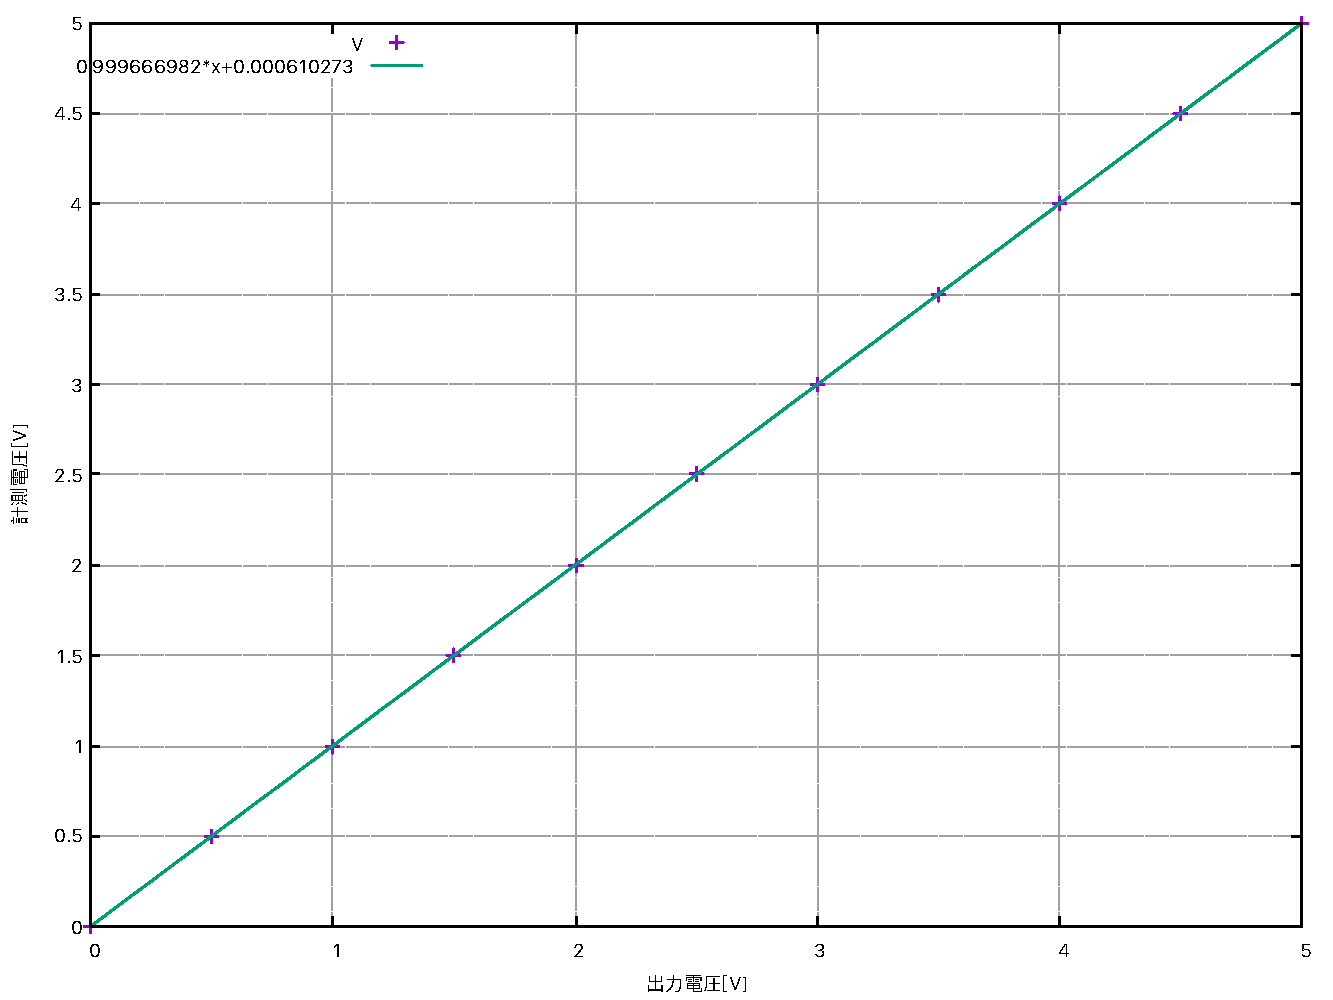
\includegraphics[scale=0.45]{./fig/RMSE.pdf}
\caption{出力電圧-計測電圧及び近似曲線}
\label{fig:RMSE}
\end{figure}
\end{enumerate}

\newpage
\begin{enumerate}[実習3-1:]
\item $R_{0}$の値を変更した時のそれぞれの電圧電流特性の傾きから抵抗値を求め.公称値と比較せよ.
また$R_{0}$の変化が算出した抵抗値にどのような影響を及ぼすのかについて考察せよ.

\wtab{sqr-R0}に,それぞれの$R_{0}$で電圧-電流のグラフ(x:電圧, y:電流)の近似直線をExcel上で最小二乗法により算出した.
傾きは\weq{1/R}で与えられるため,傾きの値の逆数をとることにより,抵抗値を求めることができる.(同表での計算値列)\\
どの$R_{0}$でも計算値の方が公称値より大きくなっていることがわかる.しかし,抵抗値によって誤差が変わり,最も誤差の大きい10\,k\rm{$\Omega$}と最小の100\,k\rm{$\Omega$}ではおよそ266\,倍もの違いがある.
そのため,測定素子や手法などによって適切な抵抗を利用する必要があるだろう.

\begin{equation}
\frac{I}{V}=\frac{1}{R}
\label{eq:1/R}
\end{equation}

\begin{table}[h]
\centering
\caption{$R_{0}$の公称値と計算値}
\label{tab:sqr-R0}
\begin{tabular}{cccc}
\hline
公称値[\rm{$\Omega$}]  & 近似直線の傾き[\rm{1/$\Omega$}]   & 計算値[\rm{$\Omega$}]  &誤差[\rm{$\Omega$}] \\
\hline
100  & 0.00999947  & 100.005298 & 0.005298412 \\
1k   & 0.000999971 & 1000.0287 & 0.028702093 \\
10k  & 0.00010     & 10000.8006 & 0.800641642 \\
100k & 0.00001     & 100000.003 & 0.003010618 \\
\hline
\end{tabular}
\end{table}
\item 各端子間のつまみ位置による電圧電流特性の変化の仕方から,使用した可変抵抗器の内部構造を予測せよ.

まず,\wfig{3-2-3}より,端子3-1間はつまみ位置に依存せず10\,k\rm{$\Omega$}となっている.(\wtab{3-1R})
次に端子1-2間は,つまみをA$\to$B$\to$Cと変化させていくと,電流が流れにくくなる.つまり,抵抗値が増加している.
また,端子2-3間は1-2間での動作と逆の動きであるため,\wfig{build}のような構造であると考えられ,\wfig{ALPS}との一致する.

\begin{table}[h]
\centering
\caption{計測値より導出される端子3-1間の抵抗値}
\label{tab:3-1R}
\begin{tabular}{cccc}
\hline
接続先&A&B&C\\
\hline
電圧[\rm{V}] & 10403.07355 &10365.33156 & 10732.50484\\
\hline
\end{tabular}
\end{table}

\begin{figure}[h]
\centering
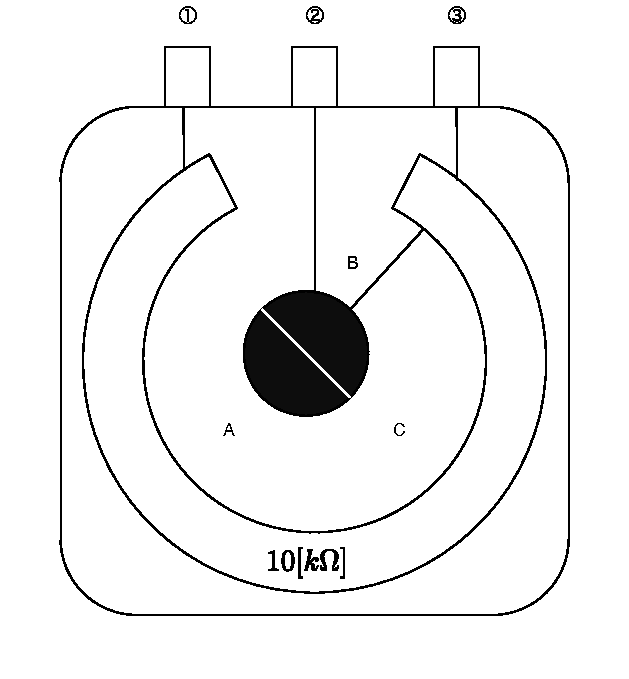
\includegraphics[scale=0.5]{./fig/build.pdf}
\caption{可変抵抗器の構造予測}
\label{fig:build}
\end{figure}

\item  電圧電流特性の変化から,CdSセンサの抵抗値と光強度の関係について考察せよ.またその(CdS セルの)原理を調査し,実験結果が正しいか確認せよ.

\wfig{3-3}より,光強度が増加すると,電流が大きくなる.つまり,抵抗値が小さくなっていることが読み取れる.この結果は原理と一致しているため,正しい結果だといえる.(参照:\ref{CDSG})

\item 電圧電流特性の変化から,力の強さに依存して力センサの抵抗値がどのように変化するか考察せよ.またその(感圧センサの)原理を調査し,実験結果が正しいか確認せよ.

\wfig{3-4}より,力が増加すると電流も増加すること,抵抗値が減少することがわかる.このことは\ref{PG}と整合性があるため,正しい結果である.

\item 発光の色が異なるということは物理量として何が異なっているのかを示し,LEDの色に応じて電圧電流特性の特徴(立ち上がり電圧,傾き)どのような違いがあるか考察せよ.

発色の色の違いは``波長''である.
参考資料として\wfig{rl}に色と波長の関係を示す.\\
\wfig{3-5}から色により,立ち上がり電圧(Forward Voltage Drop,$V_{F}$)が異なり,赤色が他の色より$V_{F}$の値が小さいことがわかる.
また,傾きも青色,白色,緑色が同じような傾き(およそ0.0005\,1/\rm{$\Omega$})をとっているのに対し,赤色はそれらより傾きが大きい値(およそ0.002\,1/\rm{$\Omega$})である.\\
ここで,光のエネルギー$W$は\weq{W}で与えられる\cite{1130000795538269056}.つまり,光の波長が長くなれば(赤外線に近づけば),エネルギーは減少するということを意味し,今回の結果はこの方程式と矛盾はない.\\
すなわち,LEDの立ち上がり電圧は赤外線に近づくほど小さくなり,傾きは赤外線に近づくほど急になるといえる.\\
また,白色LEDは\ref{LEDG}で述べたように,青色と黄色蛍光体を用いる手法と光の3原色を用いる手法があるが,今回使用したLEDはグラフ上で,赤色と緑色の中間に位置しており,可視光の中間点であるおよそ$525\,\rm{nm}$(\weq{half})に近いため,後者の手法で作成されたものだと考えられる.
\begin{align}
W=h\nu&=h\frac{c}{\lambda}\label{eq:W} \\
h:プランク定数&, \nu:振動数, c:光速\nonumber
\end{align}
\begin{equation}
\label{eq:half}
(650+400)/2=525\,\rm{nm}
\end{equation}

\begin{figure}[h]
\begin{minipage}[c]{0.5\hsize}
\centering
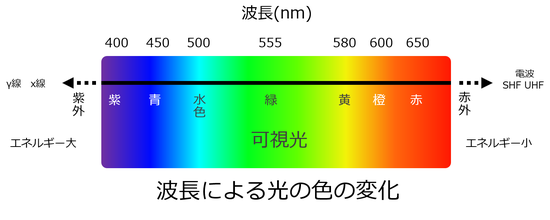
\includegraphics[scale=0.5]{./fig/波長による光の色の変化.png}
\caption{光と波長\cite{gbcalasdjdv}}
\label{fig:rl}
  \end{minipage}
  \hfill
  \begin{minipage}[c]{0.5\hsize}
    \centering
\caption{発色光の違いと素子の特徴}
\label{tab:}
\begin{tabular}{ccc}
\hline
発色光&傾き[\rm{1/$\Omega$}]&$V_{F}$[\rm{V}]\\
\hline
赤色 & 0.00118  & 15 \\
青色 & 0.000501 & 18 \\
白色 & 0.00056  & 20 \\
緑色 & 0.000533 & 19 \\
\hline
\end{tabular}
\end{minipage}
\end{figure}
\end{enumerate}

\subsection{独自考察}
\begin{itemize}
\item 0\,\rm{V}で相対誤差が他の電圧測定時と異なり誤差が大きくなったのは,実際に実験をする際にノイズなどの影響により,理論通りに0\,\rm{V}にならかったためだと思われる.よって0\,\rm{V}近傍の計測では,遅延時間の設定が他の測定電圧より長くとる必要があるのではないだろうか.
\end{itemize}